\chapter{相关工作}\label{chap:related_work}

本章首先介绍软件实现二进制翻译的相关工作,包括著名的几款二进制翻译器,如QEMU、Rosetta2、ExaGear、LATX等,
并对软件二进制翻译器的性能开销进行分析,发现间接跳转的性能开销以及指令集语义差异是其主要瓶颈。
接下来介绍软硬协同二进制翻译器的相关工作,包括超长指令字兼容和指令集扩展,能有效缓解性能开销,但仍有一定局限性。
为了解决间接跳转和指令集语义差异的问题,引出了复杂指令集x86处理器的微码缓存的概念,为微译器的设计提供了设计思路。

\section{软件二进制翻译器}

软件二进制翻译器是一种通过软件实现的二进制翻译器,
它对硬件改动较小,能够在不同的硬件平台上运行,因此具有更好的可移植性和灵活性。
本节主要介绍一款开源的用户态二进制翻译器QEMU,以及三款商用级的用户态二进制翻译器,包括苹果公司的Rosetta2、华为公司的ExaGear、龙芯公司的LATX。
其中Rosetta2和LATX也有硬件支持,但主要还是依赖软件实现,因此归类为软件二进制翻译器。

\subsection{QEMU}

QEMU是一个广泛使用的开源多平台二进制翻译框架,特别在云计算环境中,它常和KVM一起使用,提供了一种高效的虚拟化解决方案。
QEMU同时支持系统态翻译和用户态翻译,本文主要关注用户态翻译部分,它允许在一个主机操作系统上模拟另一个操作系统的应用程序。

QEMU也同时支持多种架构,包括x86、ARM、RISC-V等,使其成为开发跨平台应用程序的理想工具, 也可用于软件开发、测试以及安全研究。
如图\ref{img:qemu_arch},它通过将不同指令集的机器代码翻译成中间语言(IR,Intermediate Representation),再将IR翻译成宿主指令集,实现跨架构的兼容性。
这种设计使得QEMU能够处理多种指令集,为用户提供了一定的灵活性。然而,QEMU的性能仅能达到原生性能的10\%,
这主要归因于双层翻译(客户代码翻译到IR,IR翻译到宿主代码)的性能损失以及Helper函数模拟浮点和向量指令的性能开销\cite{deflater}。

\begin{figure}[!htbp]
  \centering
  \includegraphics[width=0.6\linewidth]{./image/qemu-IR.pdf}
  \bicaption{\enspace QEMU二进制翻译器架构图}{\enspace The architecture of QEMU binary translator}
  \fignote{通过中间代码,QEMU能在多种宿主指令集机器上运行多种客户程序。}
  \label{img:qemu_arch}
\end{figure}

基于QEMU的优化主要旨在提高其性能和执行效率,例如中间代码优化\cite{LiNan2021}、基本块链接优化\cite{Hong2012HQEMUAM}、缓存管理\cite{FengYue2010}、Helper函数优化\cite{Wang2021}等。
以下给出两个优化示例,包括HQEMU的多线程并行翻译和执行,以及寄存器分配的优化。

HQEMU\cite{Hong2012HQEMUAM}是一个基于QEMU和LLVM构建的多线程和可重定向动态二进制翻译器。
这个项目的目标是通过利用多核处理器的并行处理能力来减轻DBT的开销,同时允许更复杂的优化技术的应用。
HQEMU通过在不同的线程上分别运行QEMU翻译器和LLVM优化器,从而实现了这一目标。
在一系列基准测试中,比如SPEC CPU2006,HQEMU在x86到x86-64的模拟中,相比于原始的QEMU性能提高了2.4倍至4倍。

在动态二进制翻译中,寄存器分配是提高翻译代码执行效率的关键。原始的QEMU在许多宿主机上将所有目标寄存器映射到内存,并仅将少数临时变量存储在宿主寄存器中。
这种方法并没有考虑相邻指令之间的依赖关系,导致即使在执行前一个指令时已经将一个客户寄存器的值加载到临时变量中,执行下一个指令时也需要再次从内存中重新加载该值。
为了解决这个问题,\cite{Hong2012HQEMUAM}提出了一个优化方法,其在两个或更多相邻指令执行中有效利用了临时变量,
从而减少了对内存的不必要访问。通过这种优化,基准测试显示可以实现10\%到20\%的速度提升。

尽管以上优化示例展示了通过改进QEMU的翻译过程和内部机制,可以提升QEMU的效率和性能,
但是改进后的性能仍然仅相当于原生性能的一小部分,这在一些对性能要求较高的应用场景下显得不够可用。


\subsection{Rosetta2}

Rosetta2 是苹果公司开发的商用二进制翻译系统,
通过支持预先编译(AOT)和即时编译(JIT)两种模式实现动静结合翻译,
预先翻译对性能影响大的代码,并把翻译后代码保存在磁盘上,而对于需要动态解析的代码,采用即时编译的方式进行翻译。
Rosetta2 主要针对64位的x86\_64指令集进行翻译,以适配苹果M1等ARM64处理器的架构。

Rosetta2 的核心目标是保证MacOS上的x86软件能够在ARM架构下运行,这要求对系统调用进行转换,以匹配基于ARM的MacOS版本。
由于x86和ARM指令集都采用小端法(little-endian),这简化了指令翻译过程,避免了复杂的字节序反转操作。
这一点与苹果过去从PowerPC(大端法,big-endian)切换到x86的过程不同,后者在转换时面临更多的挑战。

然而,x86(强内存序)与ARM(弱内存序)在内存一致性模型上的差异可能导致多线程软件运行结果出现差异,这是模拟x86的一个主要挑战\cite{Risotto}。
苹果通过在芯片内部额外实现一个Intel版本的强内存TSO模型,并通过后门开关在运行Rosetta2时切换到该内存模型,解决了这一问题。
硬件支持的内存模型有效的降低来并发程序翻译的性能开销,提高了Rosetta2的性能。

\subsection{ExaGear}

ExaGear是华为公司开发的动态二进制翻译软件,专为在基于自研的ARM鲲鹏服务器上运行而设计。
ARM服务器由于其能效比优势,逐渐在数据中心中得到广泛应用,但是由于软件生态的限制,一些只有x86版本的软件无法在ARM服务器上运行。
ExaGear通过将x86应用程序翻译为ARM指令集,使得这些软件能够在ARM服务器上运行。

ExaGear通过修改Linux的binfmt\_misc组件,使得系统能够识别并使用ExaGear作为x86应用程序的解析器,实现了在安装过程中的高效集成。
ExaGear主要包括两个关键组件:指令翻译引擎和x86运行环境。指令翻译引擎充当x86应用程序与ARM架构服务器之间的中间件,实现了在x86应用程序启动时的实时翻译功能。
x86运行环境为x86应用程序提供了必要的标准库、实用程序和配置文件,构建了一个完整的运行时环境。
此外ExaGear还通过Trace优化技术来减少分支数目,进而改善内存布局和局部性,减少间接跳转查找过程\cite{LvYandong2021}。

\subsection{LATX}

龙芯二进制翻译器(LATX)是龙芯公司开发的一款动态二进制翻译软件,用于在龙芯处理器(LoongArch架构)上运行x86架构的应用程序。
结合LATX和Wine\cite{amstadt1994wine}(一 个 操 作 系 统 API翻译软件,它可以用Linux的系统调用来模拟实现Windows的系统调用,从而实现在Linux/ x86上运行Windows/x86的应用程序),
用户可以在龙芯处理器上运行大量的x86应用程序,包括Windows应用程序,例如微信、WPS、部分游戏等。

后文\ref{sec:isa_extension}节会讲解,通过添加龙芯二进制翻译扩展指令(LBT),LATX能生成出更接近x86语义的宿主指令,而无需用多条指令模拟。
此外,LATX 也添加了各类优化措施,例如x86 EFLAGS延迟计算、基本块链接、跨基本款反馈优化等,更多细节可以参考胡起的硕士论文\cite{HuQi2023}。

表\ref{tab:BTs} 对本节提到的4个主流的二进制翻译器进行了总结。

\begin{table}[!htbp]
  \centering
  \bicaption{\enspace 主流二进制翻译器}{\enspace The mainstream binary translators}
  \footnotesize% fontsize
  \setlength{\tabcolsep}{4pt}% column separation
  \renewcommand{\arraystretch}{1.2}%row space 
  \label{tab:BTs}
    \begin{tabular}{llll}
    \hline
    二进制翻译器    & 公司   & 客户平台           & 宿主平台           \\ \hline
    QEMU      & 开源项目 & x86、ARM、RISC-V等 & x86、ARM、RISC-V等  \\
    ExaGear   & 华为   & x86            & ARM            \\
    Rosetta2  & 苹果   & x86            & ARM            \\
    LoongArch & 龙芯   & x86            & LoongArch      \\ \hline
    \end{tabular}
    \end{table}

\section{软件二进制翻译的性能开销分析}\label{sec:bt_overhead_all}

\subsection{理论分析}\label{sec:bt_overhead}

在进行性能分析之前,我们可以先对二进制翻译器的性能开销进行理论分析。
如图\ref{img:bt_overhead},二进制翻译的性能开销主要分为两类:指令集语义差异和二进制翻译器机制的开销。

\begin{figure}[!htbp]
  \centering
  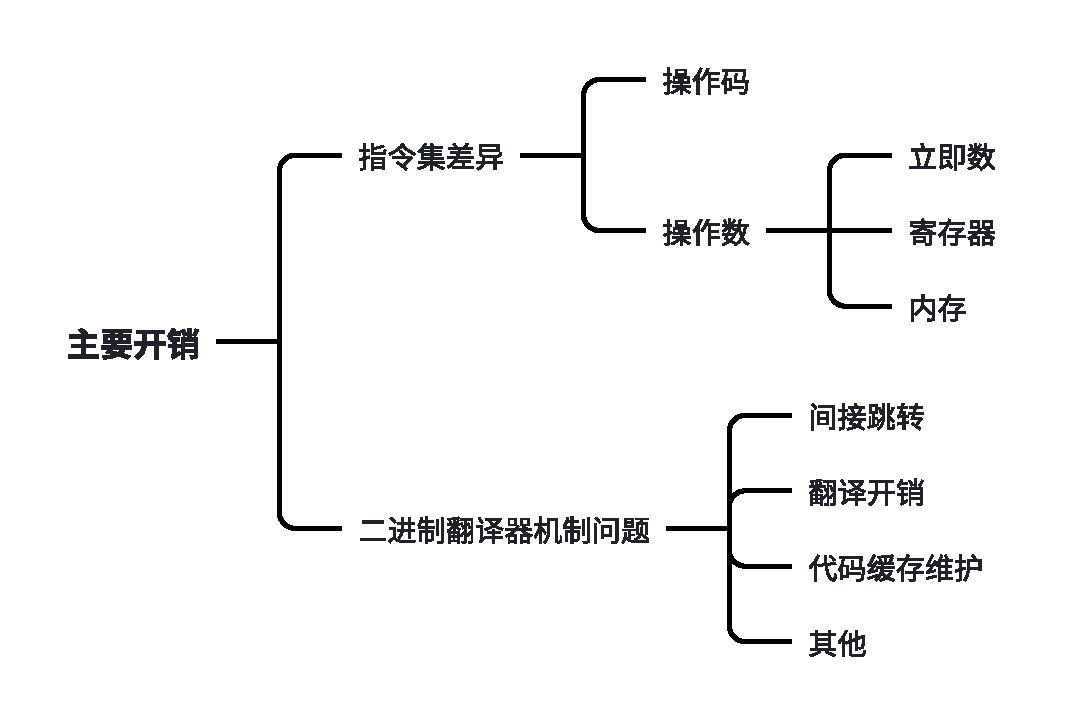
\includegraphics[width=0.7\linewidth]{./feishuImage/overhead_all.pdf}
  \bicaption{\enspace 二进制翻译器的性能开销分析}{\enspace The anaylsis of binary translator overhead}
  \label{img:bt_overhead}
\end{figure}

指令集是计算机软件和硬件交互的接口,是定义了计算机的操作和数据的格式的一种规范。
指令包括操作码和操作数,操作码是指令的功能码,操作数是指令的操作对象。其中操作数按照操作对象可以分为立即数、寄存器、内存等。
\begin{itemize}
\item 操作码不同导致一条客户指令翻译成多条宿主指令,例如乘累加指令翻译为乘法和累加两条指令。
\item 如果客户指令的立即数范围大于宿主指令的立即数范围,那么需要额外的指令来存放或加载立即数。
\item 如果客户指令的寄存器数量大于宿主指令的寄存器数量,那么需要额外的指令来保存和恢复寄存器,也称为寄存器溢出。
\item 如果客户指令的内存访问模式复杂,那么需要额外的指令来计算内存地址。
\end{itemize}

而二进制翻译器机制的开销主要包括:
\begin{itemize}
\item 间接跳转的性能开销:如图\ref{img:indirect_jump},间接跳转是指在程序运行时,通过读取寄存器的值来决定跳转到哪个地址。
这种跳转方式在静态翻译时无法确定,因此需要在运行时查询哈希表来确定跳转地址,通常需要10余拍。
\item 翻译开销:翻译开销是指动态二进制翻译器在翻译客户指令时产生的性能开销。这种开销主要包括指令翻译、基本块优化、基本块链接等。
\item 代码缓存维护: 二进制翻译器需要维护一个软件的代码缓存,用于存储翻译后的宿主指令。当缓存满时,需要进行缓存替换产生开销。
\end{itemize}

\begin{figure}[!htbp]
  \centering
  \includegraphics[width=0.6\linewidth]{./image/indirect_jump.pdf}
  \bicaption{\enspace 间接跳转开销}{\enspace The overhead of indirect jump}
  \fignote{由于翻译后的代码地址发生了非线性偏移,间接跳转的目标地址只能在运行时查询哈希表获取,通常需要10余拍\cite{dantrasOptimizingIndirectBranches2016}。}
  \label{img:indirect_jump}
\end{figure}

\subsection{实验分析}

上一节提到的商用级用户级二进制翻译器,包括苹果公司的Rosetta2、华为公司的ExaGear、龙芯公司的LATX,
在运行SPEC2017基准测试时,根据\ref{eq:bt_performance}公式,得到的翻译性能分别为67.2\%、72.7\%和60\%,
距离原生性能100\%还有较大的差距,为此希望通过实验分析找出二进制翻译器的性能瓶颈。


根据本团队之前完成的一项工作\cite{deflater},基于如下两个前提,使用指令膨胀率来分析二进制翻译器的性能开销。
\begin{enumerate}
\item  为了保证客户程序的精确异常,二进制翻译器不会做指令重排这样的激进优化,即保持指令的顺序不变,指令的边界不被打破。
\item  主流二进制翻译器在运行SPEC 2017这类运算密集型的基准测试时,98\%的时间都在执行生成的宿主指令上,翻译开销
和维护代码缓存的开销可以忽略不计。
\end{enumerate}

指令膨胀率是指,每条客户指令平均翻译出的宿主指令数,是一个大于1的小数,计算方式参考\ref{eq:insts_inflt}。
举例来说,一条x86的add指令可能翻译成LoongArch的load指令和一个add指令,那么这条x86 add指令的膨胀率就是2。
对所有的客户指令的膨胀率求加权平均值,权重为客户指令的动态执行次数,即得到了某个翻译器在运行某个程序的指令膨胀率
(为了说明简单,忽略了基本块内指令的优化)。

\begin{equation}
  \text{总体膨胀} = \frac{\text{生成的宿主指令数}}{\text{客户指令数}} \\
  = \frac{\sum_i \text{指令频次}_i \times \text{指令膨胀率}_i}{\sum_i \text{指令频次}_i}
  \label{eq:insts_inflt}
\end{equation}

假设所有指令执行时间相同,那么膨胀了多少倍,程序的执行时间就会变长多少倍。
事实上,不同指令的执行时间是不同的,但可以大致通过指令膨胀率来估计程序的性能开销。
指令膨胀率越高,翻译后的程序要执行的指令数越多,执行时间越长,性能越低。即便多发射处理器能在单拍内执行多条指令,缓解更多指令带来的性能开销,
但根据测试数据,指令膨胀率和性能下降值保持正相关,相关系数为0.98\cite{deflater}。因此,可以用指令膨胀率来衡量性能开销。


\begin{figure}[!htbp]
  \centering
  \rotatebox{90}{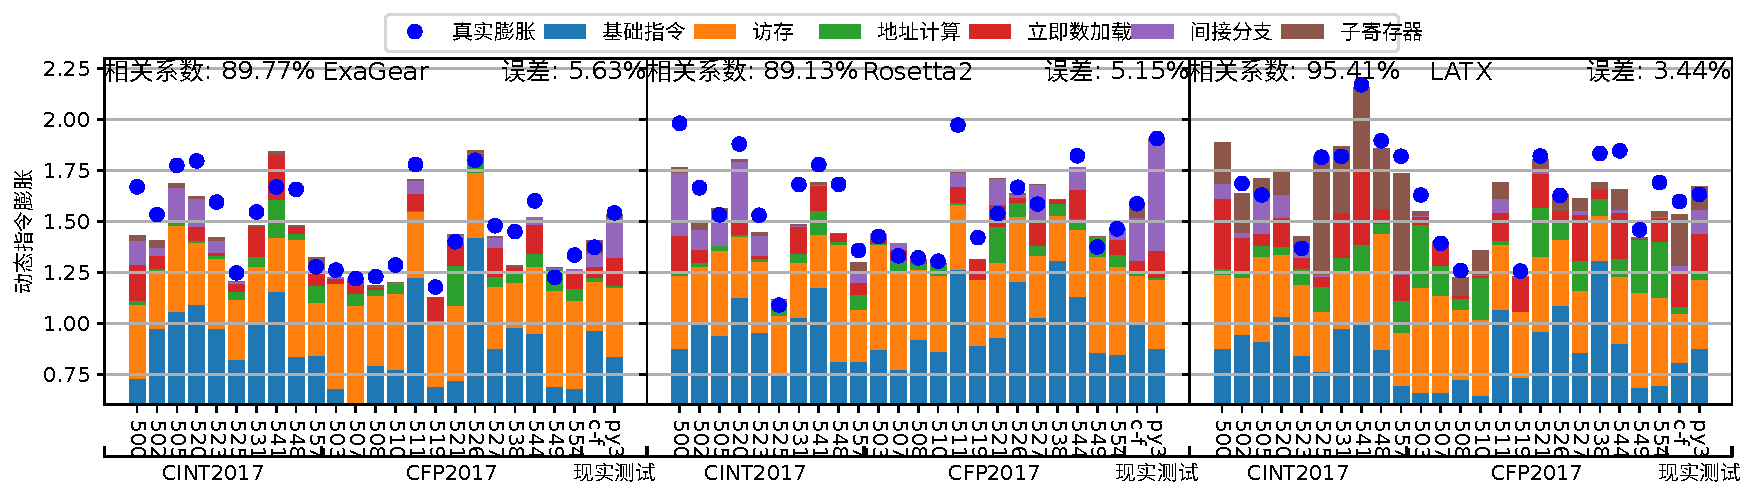
\includegraphics[width=\textheight,height=\textwidth,keepaspectratio]{./plot_pdf/insts_inflt_breakdown_2017.pdf}}
  \bicaption{\enspace 三个主流二进制翻译器指令膨胀来源分析图\cite{deflater}}
      {\enspace The breakdown of instruction inflation for three major binary translators\cite{deflater}}
  \label{img:insts_inflt_breakdown_2017}
\end{figure}

如图\ref{img:insts_inflt_breakdown_2017},
测量并模拟了3款商用级二进制翻译器(ExaGear、Rosetta2、LATX)在运行SPEC2017的指令膨胀率,模拟误差在5\%以内。
注意这三款翻译器都是复杂指令集(x86)到精简指令集(ARM/ LoongArch)的翻译器,这两类指令集语义差异较大,因此指令膨胀率较高。
图中\ref{img:insts_inflt_breakdown_2017}蓝色的点表示测量的真实膨胀率,而分解成不同颜色的柱状图表示模拟的膨胀率来源。
根据指令膨胀率的来源,主要将开销分成了5类:


%latex 使用1. 2. 3. 来编号
\begin{enumerate}
  \item \textbf{指令集间操作码差异:} 不同指令集的操作码差异引起Eflags计算等操作的额外指令翻译,增加了指令膨胀率。此外LoongArch对于子寄存器默认符号扩展,x86/ARM默认零扩展。对应图\ref{img:insts_inflt_breakdown_2017}中\textcolor{Sepia}{\textbf{棕色}}部分。
  
  \item \textbf{操作数访问模式不同:} 复杂指令集(x86)可以直接访问内存,而其他精简指令集只能操作寄存器,导致操作数模式不同。对应图\ref{img:insts_inflt_breakdown_2017}中\textcolor{orange}{\textbf{橙色}}部分。
  
  \item \textbf{地址计算不同:} 复杂地址计算方式(x86)与其他指令集的简单计算方式导致在翻译时需要额外指令。例如x86计算地址$addr = base + index * scale +disp$; 其他的大多为$addr = base + offset$。 对应图\ref{img:insts_inflt_breakdown_2017}中\textcolor{green}{\textbf{绿色}}部分。
  
  \item \textbf{立即数加载:} x86是变长指令集,支持编码64位立即数和32位地址偏移;而其他指令集均为定长指令集,立即数的编码空间有限。在翻译一条带有长立即数的指令时,需要额外的访存指令(从内存加载长立即数)或者是多条立即数加载指令(多个短立即数拼接成一个长立即数)。对应图\ref{img:insts_inflt_breakdown_2017}中\textcolor{red}{\textbf{红色}}部分。
  
  \item \textbf{间接跳转:} 客户指令地址到宿主指令地址是非线性的,而间接跳转的目标地址在运行时才能知道,需要额外的几条指令查询间接跳转哈希表,导致性能开销。对应图\ref{img:insts_inflt_breakdown_2017}中\textcolor{Purple}{\textbf{紫色}}部分。
  
\end{enumerate}

以上五类主要开销也对应于上一节\ref{sec:bt_overhead}理论分析的内容:
前4个属于指令集语义差异,分别对应操作码、内存、立即数开销(操作数访问模式不同也属于复杂指令集和精简指令集的差异,也可归为操作码不同);而间接跳转属于二进制翻译机制问题。
由于x86\_64通用寄存器只有16个,少于ARM/LoongArch的32个通用寄存器,所有没有寄存器溢出产生的开销。
而翻译开销和代码缓存维护的开销在现代高性能二进制翻译器中也是可以忽略不计的。

以上这5类主要开销总结起来,主要包括\textbf{指令集语义差异}和\textbf{间接跳转开销}这两个方面,其性能开销
很难通过软件优化来解决,接下来将介绍软硬协同二进制翻译器的相关工作。

\section{软硬协同二进制翻译器}

指令集作为软件和硬件沟通的桥梁,设计初衷是让软件和硬件设计解耦,使得软件开发者不需要关心硬件的细节,只需要关心软件的逻辑。
而二进制翻译器则是一种将不同指令集之间的桥梁,它可以将不同指令集的二进制代码翻译为目标指令集的二进制代码,从而实现不同指令集之间的兼容。
从设计层次来看,二进制翻译器相对指令集更加靠近硬件层,因此添加硬件支持的软硬协同二进制翻译器是一个比较自然的选择。

此外,二进制翻译器一般应用于生态迁移,在处理器厂商推出新型处理器时,为了保持对旧软件的兼容性,或者引入其他指令集已有的繁荣生态,需要引入二进制翻译器。
处理器厂商也有动力在新型处理器中添加硬件支持,以提高二进制翻译器的性能,减少软件兼容的性能开销。
本节主要介绍两个代表性的软硬协同二进制翻译器,分别是Transmeta公司的超长指令字兼容和龙芯公司的指令集扩展技术。

\subsection{超长指令字}

在处理器设计早期,由于当时的硬件晶体管资源有限,难以硬件发掘指令集并行性,因此超长指令字(Very Long Instruction Word, VLIW)技术应运而生。
超长指令字技术通过软件来发掘指令级并行性,将多条指令打包成一条超长指令字,从而提高指令级并行性,提高处理器的性能。
Transmeta公司推出的Crusoe处理器就是一种基于超长指令字的处理器,其宣称在性能和功耗方面都优于同期的x86处理器\cite{dehnertTransmetaCodeMorphing2003}。

但由于初期超长指令字技术的复杂性和软件开发者对于超长指令字的不熟悉,导致超长指令字生态并不繁荣,
因此Transmeta公司配套推出了软件上的代码转换器(Code Morphing Software, CMS),通过软硬协同的方式实现了对x86指令集的兼容。
Transmeta的CMS充当了翻译器和优化器的角色,使得基于非x86的VLIW处理器能够执行x86二进制代码。
还提供了一个动态优化的执行环境,能够在运行时对代码进行优化,从而提高执行效率和能耗性能\cite{dehnertTransmetaCodeMorphing2003}。

如图\ref{img:transmeta_arch}所示,代码转换器将从程序接收到的x86汇编代码指令翻译成微处理器的本机指令(超长指令字)。
通过这种方式,Crusoe 也可以模拟其他指令集架构,例如Crusoe 也能将字节码翻译为其本机指令集中的指令来执行 Java 字节码。

\begin{figure}[!htbp]
    \centering
    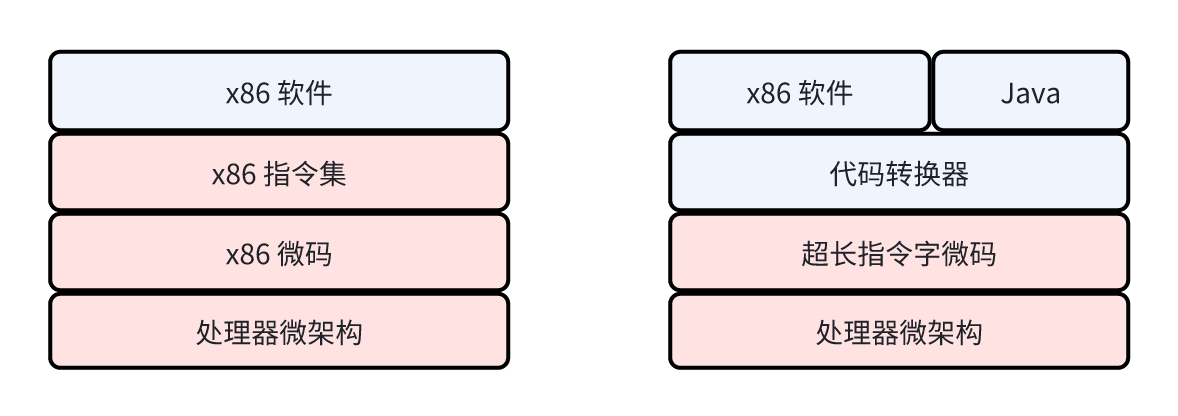
\includegraphics[width=0.8\linewidth]{./feishuImage/transmeta_arch.png}
    \bicaption{\enspace Transmeta架构图}{\enspace The architecture of Transmeta}
    \fignote{在超长指令字处理器上实现兼容x86的指令集,并支持JAVA程序。}
    \label{img:transmeta_arch}
  \end{figure}
这种架构有如下特点:

\begin{itemize}
\item 架构兼容性与灵活性:Transmeta从初代128位VLIW处理器切换到第二代的256位VLIW处理器,都能通过软件翻译器保持软件向前兼容。
\item 解释与翻译配合:冷客户代码通过解释执行,热代码通过翻译执行,提高了执行效率。
\item 精确异常处理:Transmeta在硬件中引入了一套提交和回滚机制,当发生异常时,配合软件翻译器回滚,能够保证异常处理的精确性。
\end{itemize}

尽管Transmeta公司提出了许多创新的技术,但并未在市场上取得成功,最终于2007年退出处理器市场。
随着半导体工艺进步,处理器的晶体管资源变得丰富,基于硬件的乱序执行技术逐渐成熟,已经能够用硬件发掘指令级并行性,
超长指令字技术的优势逐渐减弱,超长指令字技术的发展也逐渐停滞。
但Transmeta公司在多架构兼容性方面的工作提供了宝贵的经验,成为软硬结合二进制翻译器的重要先驱者。

\subsection{指令集扩展}\label{sec:isa_extension}

客户和宿主指令集语义差异是二进制翻译器性能的主要瓶颈之一,为了解决这个问题,在宿主指令集中添加指令集扩展来接近客户指令集的语义是一种常见的解决办法。
例如龙芯公司在LoongArch指令集中添加的二进制翻译扩展指令(Loongson Binary Translation, LBT)\cite{LoongArch2023}。

龙芯早期使用MIPS指令集,并添加了便于x86和ARM二进制翻译的一系列自定义指令集,例如对x86 EFLAGS的支持、对X87浮点指令的支持、非对齐访存的支持等,形成了LoongISA\cite{LoongISA}。
但由于MIPS中用户定义指令(UDI,user defined interface)槽位有限,导致了LoongISA的指令集扩展受限,
所以在2020年龙芯公司发布了全新的、自主可控的、支持更多指令集扩展的LoongArch架构\cite{LoongArch2023}。
并从3A5000开始,龙芯处理器开始支持LoongArch架构,并配套使用LATX二进制翻译器进行x86应用程序的翻译。
LoongArch指令集中包括了对二进制翻译支持的扩展指令集,称为LBT指令集,用于支持x86、ARM、MIPS的二进制翻译。
LBT扩展指令集与LATX软件配合使用,可以实现更高效的二进制翻译,提高了龙芯处理器的软件兼容性。

指令集扩展虽然能够接近客户指令集的语义,但这样会增加宿主指令集的复杂度,更加剧了指令集的历史包袱,同时添加指令集扩展也难以支持多种指令集的兼容。


% \section{x86 微码缓存的相关工作}
\section{x86处理器微码缓存}\label{sec:complex_isa}

x86 微码缓存(Uop Cache)
是为了在 x86 CPU 后端实现超标量乱序执行并降低译码功耗而引入的关键组件\cite{solomonMicrooperationCachePower2001},
本节对其介绍。

\subsection{微码缓存介绍}

x86处理器是一种复杂指令集计算机,其指令集架构复杂,指令长度不固定,指令格式多样。
为了实现超标量乱序执行,x86 CPU 后端需要将复杂的变长x86指令转换成类RISC格式的定长微码。
微码的引入简化了指令集的关系,降低了CPU后端设计复杂度,使得指令能在后端能够更高效地乱序执行。

为了降低译码能耗、提高性能,研究者们引入了微码缓存,用于存储已经译码过的微码。
如果这条指令已经译码过,就直接从微码缓存中读取微码,而不需要再次译码。
\cite{solomonMicrooperationCachePower2001}论文中指出,在标准测试集中,
微码缓存能消除75\%的指令译码,在多媒体应用中,这个比例甚至高达90\%。
对于Intel P6处理器来说,能节省10\%左右的整机功耗。

\begin{figure}[!htbp]
  \centering
  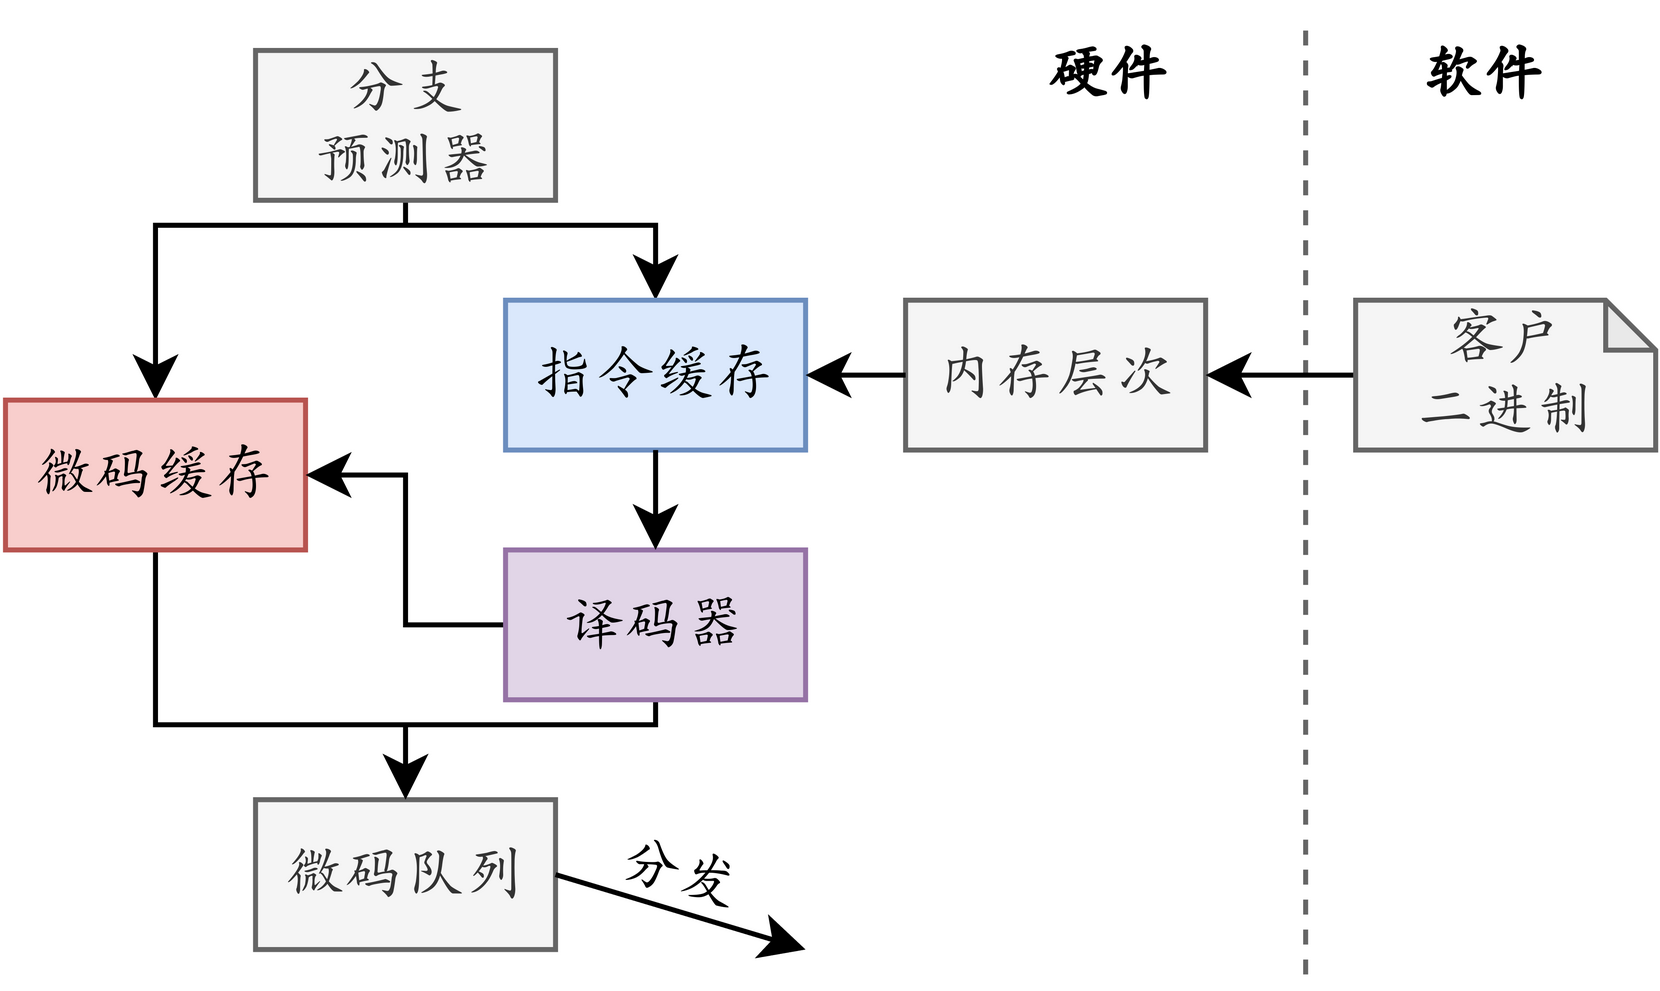
\includegraphics[width=0.6\linewidth]{./image/front_end_ucache.pdf}
  \bicaption{\enspace x86处理器前端架构图}{\enspace The architecture of x86 processor front end}
  \fignote{前端包括指令缓存和微码缓存。
  如果微码已在微码缓存中则直接使用;如果微码未缓存则从指令缓存中取得指令,进行译码并存入微码缓存中。}
  \label{img:front_end_ucache}
\end{figure}

具体而言,在CPU的前端,指令缓存和微码缓存是分开的,如图\ref{img:front_end_ucache}。
在前端译码阶段,系统会首先查询微码缓存,检查是否已经缓存了当前指令的微码。
如果微码已经在缓存中,CPU 就直接读取微码并发射到后端执行。
如果微码未缓存,系统则从指令缓存中取得指令,进行译码,并将译码结果存入微码缓存中,注意一个指令缓存行可能生成多个微码缓存行。

\subsection{微码缓存组织形式}

微码缓存的组织形式与指令缓存有所区别。指令缓存的地址被分为标记、索引和块偏移三部分,而微码缓存的地址被分为标记、索引两部分,其中地址低位的块偏移也是标记的一部分。
这是因为一条指令会被译码为多条数量不定的微码,原本的块偏移无法唯一标识一条微码。
多条指令组成的指令基本块(以控制流指令结尾)译码成的多条微码,会尽可能放在一个微码行中,然后用指令基本块的首地址来索引这个微码行。

\begin{figure}[!htbp]
  \centering
  \includegraphics[width=0.8\linewidth]{./image/ucache.pdf}
  \bicaption{\enspace 微码缓存的组织形式}{\enspace The organization of uop cache}
  \label{img:ucache}
\end{figure}

如图\ref{img:ucache},指令地址首先通过索引找到对应的微码组,然后通过标记找到对应的微码行。
微码行开头有元信息存储有关这个微码行的信息,例如微码数量、立即数数量等。接下来读出对应的微码,发射到后端执行。

\begin{figure}[!htbp]
  \centering
  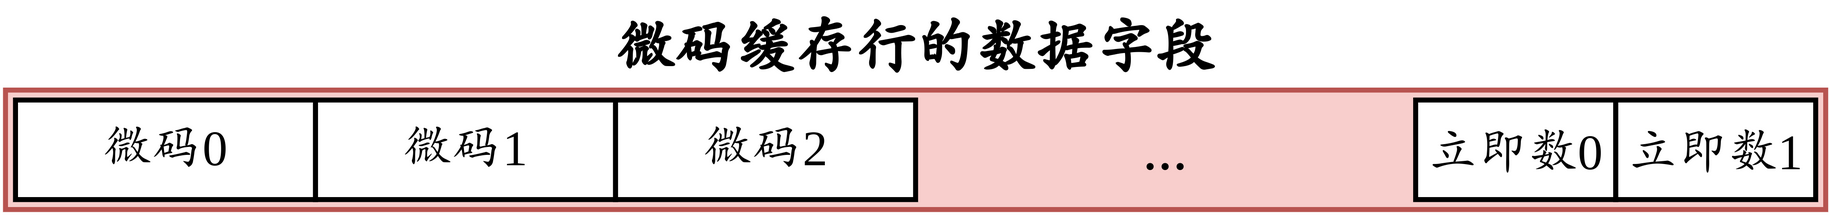
\includegraphics[width=0.8\linewidth]{./image/ucache_line.pdf}
  \bicaption{\enspace 微码缓存一行的内容}{\enspace The content of a uop cache line}
  \label{img:ucache_line}
\end{figure}

由于x86是变长指令集,微码是定长指令集,如果x86指令中有长立即数,没办法存放在定长的微码中,所以长立即数
会单独放在微码行的最后。
如图\ref{img:ucache_line},微码行中
微码和立即数是相向生长的,微码从前往后,立即数从后往前,如果相遇,说明微码行已满,需要分配新的微码行。


\subsection{微码缓存行的结束条件}\label{sec:ucache_end}

和指令缓存不同,指令缓存行是以单条指令为单位,一行会存储多条指令,没有空洞。
而微码缓存行是以基本块为单位,一行存储一个基本块的微码,存储的微码数量不固定,当基本块短时,可能会有空洞。

微码指令会尽可能填满一个微码缓存行,但是当满足如下3个条件之一时,会结束当前微码缓存行的填充\cite{solomonMicrooperationCachePower2001}:
\begin{enumerate}
  \item 遇到控制流指令并预测会跳转:当遇到控制流指令时,微码缓存会截断这一行,确保每个微码缓存行只包含一个基本块的微码。
  \item 微码缓存行已满:当微码缓存行中微码或者立即数填满一行时,会结束当前微码缓存行的填充。
  \item 遇到指令缓存行的结尾:这样保证一个指令缓存行产生的多个微码缓存行会放在同一个微码缓存组中(不同路),
  当需要刷新这一行指令缓存时, 可以方便的通过索引找到对应的微码缓存组进行刷新,而不必刷新整个微码缓存。
\end{enumerate}

此外,为了保证精确异常处理,
需要保证一条宏码对应的多条微码一起提交,在后端重排序缓冲区(ROB)中需要添加对应的标志位,标记这些微码是一起提交的。
(例如一条复杂的x86指令可能会翻译成多条微码,这些微码在后端原子化提交)。

\begin{figure}[!htbp]
  \centering
  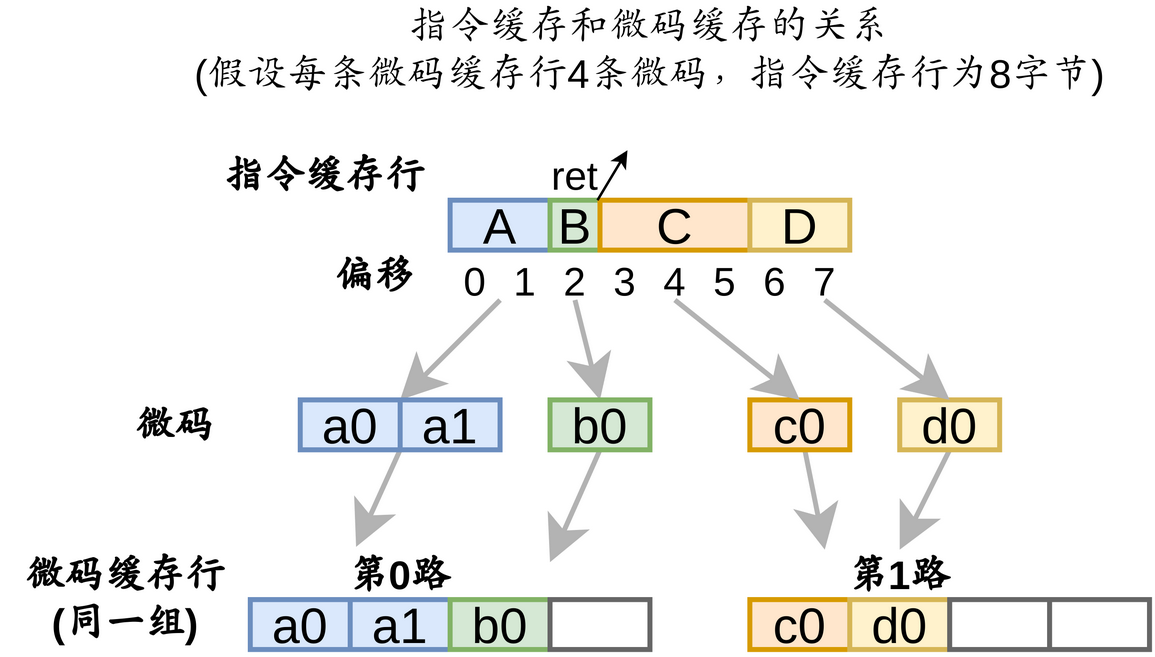
\includegraphics[width=0.8\linewidth]{./image/IC-to-UC.pdf}
  \bicaption{\enspace 指令缓存和微码缓存关系}{\enspace The relationship between instruction cache and uop cache}
  \label{img:IC_to_UC}
\end{figure}

如图\ref{img:IC_to_UC}给出了一个指令缓存行对应多个微码缓存行的示例(这里的微码行忽略了立即数的存储)。
假设指令缓存行为8字节,存储了A、B、C、D四条指令,长度分别为2、1、3、2字节,微码缓存行最多能存储4条微码。
4条指令译码得到的微码分别为a0、a1、b0、c0、d0。
则微码缓存行1存储了a0、a1、b0,微码缓存行2存储了c0、d0。
本来c0是可以存储在微码缓存行1中的,但是由于B指令是控制流ret指令,满足结束条件1,所以微码缓存行1结束,c0存储在微码缓存行2中。
可以看到结束条件导致了微码缓存行中存在空洞。

此外微码缓存行1和微码缓存行2是存放在同一个微码缓存组中不同路上的,意味着它们的索引相同,但是标记不同。
当这一个指令缓存行需要被刷新,可以通过索引找到这这一组的所有微码缓存行一起刷新,而无需刷新整个微码缓存,保证了指令缓存行和微码缓存行的一致性。

x86 微码缓存的引入为 x86 架构的超标量乱序执行提供了重要支持,
存储已经译码过的微码而无需再次译码,减少了译码的开销,降低了整体功耗。

\subsection{微码与二进制翻译相似性}

本文发现,面向x86的二进制翻译与x86处理器的微码有一定的相似性,具体表现在以下几个方面:

\begin{enumerate}
\item 面向x86的二进制翻译会在软件层将复杂的x86指令翻译成宿主指令(通常为定长的RISC指令),
而x86处理器前端在硬件层将x86指令翻译成类RISC的定长微码。
\item 二进制翻译中使用软件层的代码缓存存储翻译后的宿主指令,
而x86处理器使用微码缓存存储译码后的微码。
\item 二进制翻译可以添加指令集扩展来缩小和客户指令语义差异,
而x86处理器也可以不断修改内部的微码来适应新的x86指令集扩展。
\end{enumerate}

此外,硬件实现的微码相对于二进制翻译器还有如下优势:

\begin{enumerate}
\item 语义差异:内部的微码修改不会对外暴露,而指令集扩展技术会增加指令集的历史包袱。
\item 间接跳转开销:硬件的微码缓存维护好了x86宏码地址和微码的映射关系,没有间接跳转开销;而二进制翻译器中处理间接跳转的开销较大。
\item 精确例外处理:硬件后端ROB维护了微码的提交顺序,保证了精确异常处理;而二进制翻译器中需要额外的回退机制来保证精确异常处理。
\end{enumerate}


\section{微译器设计与实现}\label{chap:MUT}

前文\ref{sec:bt_overhead_all}通过分析发现二进制翻译器的主要开销来源于指令集语义差异和间接跳转开销。

指令集语义差异的一种常见的解决办法是在宿主指令集中添加指令集扩展,来接近客户指令集的语义,例如LoongArch指令中添加的二进制翻译扩展指令(Loongson Binary Translation, LBT)\cite{LoongArch2023}。
但这样会增加宿主指令集的复杂度,更加剧了指令集的历史包袱,同时添加指令集扩展也难以支持多种指令集的兼容。
本课题从x86处理器定义的微码指令集中得到启发,微码是一种内部指令集,不对外暴露给用户和编译器,并且可以随着处理器的演进而不断迭代优化,不需要考虑历史兼容包袱。

通过定义一套\textbf{融合微码},作为一种内部指令集,包含各个指令集的并集,对外不暴露给用户,而是通过二进制翻译器将客户指令翻译为融合微码指令,从而实现多指令集的兼容。
在这个层面上,二进制翻译器类似于一个软件译码器,将客户指令翻译为融合微码指令,而CPU则类似于一个虚拟机,执行融合微码指令。
由于x86授权问题,直接做一个硬件译码器对外支持x86指令集是不现实的,因此通过软硬协同的方式,软件的二进制翻译器将客户指令翻译为融合微码指令,再由硬件执行融合微码指令。

而对于间接跳转开销,x86的微码缓存天然的就能解决这个问题,因为硬件上的微码缓存维护好了x86指令地址和微码指令地址的映射关系,
可以通过简单的查询缓存访问到微码指令地址,
而不需要软件上复杂的哈希表查询逻辑,这样可以大大减少间接跳转的开销。
因此参考x86的微码缓存,本课题提出了一种\textbf{翻译缓存}的概念,用于存储预翻译的融合微码指令集。
% 一条x86指令译码为多条微码指令,这个和一条宿主指令翻译为多条客户指令类似,都是一种一对多的关系。

总结起来,通过借鉴x86微码和微码缓存的概念,谢本壹博士提出了一种多架构软硬协同的二进制翻译技术——\textbf{微译器},
通过\textbf{融合微码}缩小了指令集语义差异,
通过\textbf{翻译缓存}来消除间接跳转开销,提高了二进制翻译器的性能,
详细工作可参考其博士论文\cite{xieby2024}。

\subsection{微译器整体架构}

\begin{figure}[!htbp]
  \centering
  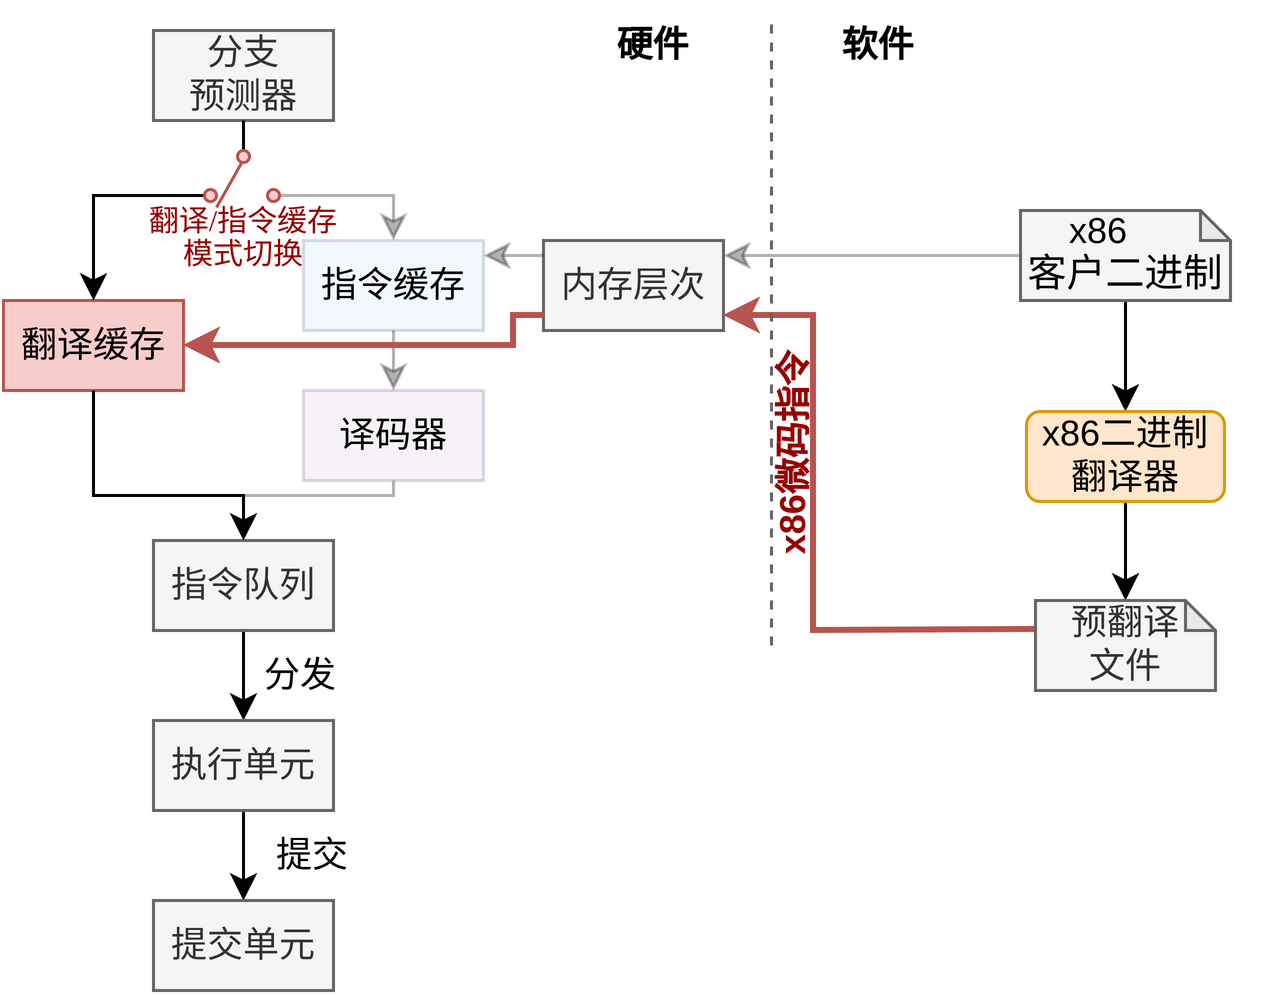
\includegraphics[width=0.8\linewidth]{./image/front_end_transutor.pdf}
  \bicaption{\enspace 微译器整体架构图}{\enspace The overview of the micro-translator architecture}
  \label{img:front_end_transutor}
\end{figure}

如图\ref{img:front_end_transutor}展示了微译器的整体架构,相对于传统的x86处理器前端图\ref{img:front_end_ucache},微译器在硬件侧和软件侧都做了一些改动。

% \subsection{硬件部分}

在硬件部分,引入了\textbf{翻译缓存}(Translation Cache),该缓存作为一级缓存负责存储预翻译的微码指令集,替代了原本的微码缓存。
翻译缓存的每行组织形式和微码缓存类似,都是前面部分存放微码指令(这里为融合微码指令,下一节详细介绍),
后面存放立即数,微码指令和立即数相向生长,中间可能有空洞,产生新的开销,后文会提出对应的优化方案。

此外与传统微码架构不同,微码缓存数据是直接来源于CPU和指令缓存,通过硬件译码器进行译码并存入微码缓存中;
而翻译缓存通过软件的二进制翻译“译码”,透过内存层次(从内存加载到L3 Cache, 再到L2Cache, 最后到微码缓存)进行填充,
取代了传统的指令缓存和译码器的角色。
在传统x86架构下,取指部件会同时查询指令缓存和微码缓存;
而在微译器架构下,取指部件仅查询翻译缓存,硬件的译码器被软件的二进制翻译器取代。
为了兼容传统的x86处理器模式,添加了一个模式切换逻辑,可以切换回使用硬件译码器进行译码,这样可以在不改变原有x86处理器的基础上实现微译器的功能。
后文默认使用软件二进制翻译器进行译码,也就是翻译缓存的方式。

% \subsection{软件部分}

在软件部分,引入了静态和动态二进制翻译器。
程序首先通过静态二进制翻译器被翻译成融合微码指令,并被写入预翻译文件,存储在硬盘中。
在客户程序执行阶段,预翻译文件被加载到内存中,程序计数器被设置为客户程序的入口。
取指部件从翻译缓存中取指,若翻译缓存或内存层次命中,则从翻译缓存取指,发送到处理器后端执行,不断取指执行。
若翻译缓存和内存层次均未命中(例如存在自修改代码等),说明客户指令还未翻译,此时会调用动态二进制翻译器进行实时翻译,
并将翻译结果写入翻译缓存,再取指执行。

接下来详细介绍微译器各个组成部分的设计与实现,包括融合微码、翻译缓存、预翻译文件、二进制翻译器。

\subsection{融合微码}\label{sec:tisa}
本节详细介绍重要的一个概念——融合微码。“融合”代表它能融合了多种指令集的特征,
包括x86和RISC-V,未来还可以支持ARM,MIPS等其他指令集,
或许叫统一微码也更好理解。但融合并非简单的把所有指令集简单拼接就好,这会造成指令集冗余,挤占有限的编码空间。
而是需要对各个指令集的特征进行分析,找到共性,抽象出一种更加简洁的指令集,这就是融合微码的设计思想。

“微码”这个名字主要由于它在翻译缓存中的组织形式和传统的x86微码缓存组织形式类似,并且更像是不同指令集的更低级表现形式;
此外目前第一代的融合微码是在原有的Gem5 x86微码上扩充的,
所以便于理解仍然保留融合微码的名字。

但事实上,融合微码有很大特征很像一个“RISC指令集”。
由于融合微码指令是需要存储在磁盘中的,并不像传统x86微码只是作为一个“暂时指令”存在于CPU运行期间,
所以融合微码指令需要像普通指令集一样进行\textbf{编码},
二进制翻译器把指令\textbf{编码}为定长的融合微码指令,并存储于磁盘中。
CPU再从磁盘中加载融合微码指令,\textbf{解码}为CPU识别的信息,这一阶段也叫“译码阶段”。
因此从这个角度来说,加上指令定长、只能操作寄存器、指令间关系被简化等特征,融合微码很像一个普通的“RISC指令集”。
因此融合微码类似传统指令集概念,也是有编码空间的概念。

\subsection{翻译缓存}\label{sec:tcache}

本节讲解翻译缓存的设计与实现,翻译缓存是微译器的核心组件,用于存储预翻译的融合微码指令集。

翻译缓存的结构整体和微码缓存类似,但是有一些细节上的差异,在此详细介绍翻译缓存行的组织形式,
重点关注元信息和数据部分,其余的标签、有效位等部分和普通的一级缓存类似。
一篇关于微码缓存的专利\cite{uopPatent}中提到了微码缓存的一行设置为74byte。
而本文设计的翻译缓存行的大小为64字节,结构类似图\ref{img:ucache_line},但是元信息部分有所不同。

\begin{figure}[!htbp]
  \centering
  \includegraphics[width=1\linewidth]{./image/tcache_line.pdf}
  \bicaption{\enspace 翻译缓存行组织形式}{\enspace The organization of the translation cache line}
  \label{img:tcache_line}
\end{figure}

如图\ref{img:tcache_line},展示了翻译缓存行的组织形式,主要对元信息部分进行了详细介绍。
翻译缓存行的大小为64字节,
前16字节存放元信息,元信息细分为两部分,第一字节存放这一行的元信息,包括这一行是否有效,对应多少条宏码指令(这里的宏码就是客户指令,用宏码是为了和微码做对应)。
接下来15字节存放每条宏码的元信息,最多可以存15条宏码指令,宏码指令元信息包括宏码指令的长度(x86指令是变长指令,存储长度来索引到下一条x86指令地址),这条宏码生成的微码数量。
最后的48字节存放微码指令和立即数,微码指令和立即数都是定长的,单位为4字节。微码指令和立即数相向生长,中间可能有空洞。

存储行信息、微码指令、立即数是十分必要的,而存储宏指令元信息是为了支持二进制翻译器中精确异常处理。
精确异常处理是指在异常发生时,这条宏指令之前的所有指令都已经执行完毕,这条宏指令之后的所有指令都没有执行。
因此需要把一条宏指令对应的几条微码看做一个整体,可以乱序执行,但是在提交阶段需要保证这几条微码指令是原子提交的。
这样就能保证精确异常处理,这也是二进制翻译器必须要支持的功能。
因此在宏指令元信息中,需要存储一条宏指令对应的微码数量信息,而宏码长度信息则为了取到下一行微码缓存行。


\subsection{预翻译文件}\label{sec:aot}

本节讲解预翻译文件(Ahead-of-Time, AOT)的设计与实现,预翻译文件是存储预翻译的融合微码指令集的文件,是静态二进制翻译器的输出。

预翻译文件的设计思想在于,尽可能多的存储所有可能用到的融合微码指令,减少动态二进制翻译的开销。
由于融合微码和普通指令在一级缓存中寻址模式不同,普通指令能根据行内偏移直接访问到指令,而融合微码只能根据行内第一条指令的地址访问到整行指令(在\ref{sec:complex_isa}小节有提到)。
也就是说,融合微码只能以一个微码行(一个基本块)为单位进行访问,而不能以一个微码指令为单位进行访问。
如果出现了跳转到一个微码行的中间位置,那么就需要重新翻译这个微码行,这样会增加额外的开销。
对于传统的x86处理器模式,这个开销是很小的,因为是硬件来译码并填充到微码缓存中,只需要2拍左右;
而对于微译器架构,这个开销就会很大,因为需要调用软件的二进制翻译器进行实时翻译,可能需要上百拍的开销,这样的开销是无法接受的。
因此提出了\textbf{重复存储}的概念,即存储任意一个地址开始的融合微码指令,这样就能保证在跳转到任意一个地址时,都能从预翻译文件中加载对应的融合微码指令。


\subsection{二进制翻译器}

软件端的二进制翻译器分为静态二进制翻译器和动态二进制翻译器,静态二进制翻译器用于将客户程序翻译为融合微码指令,并存储在预翻译文件中;
动态二进制翻译器用于在翻译缓存未命中时实时翻译客户指令。

对于动态二进制翻译器,它的基本功能是在翻译缓存未命中时实时翻译客户指令,它和静态二进制翻译器的功能类似,
只是触发时机不同,因此我们可以复用静态二进制翻译器的代码,只需要添加一个触发机制即可。
它有两个触发机制,一个是代码发现没有发现的代码,需要实时翻译;一个是由于自修改代码等原因,翻译缓存行失效,需要实时翻译。
具体在硬件上,当翻译缓存行失效时,会触发例外(类似缺页异常),这时会调用动态二进制翻译器进行实时翻译,将翻译结果写入翻译缓存。


\section{本章小结}

% 本文采用了硬件辅助的策略。其中,一些关键的工作包括:

% 1. 融合微码以缩小指令集语义差距: 针对指令集间操作码差异、操作数据模式不同以及地址计算不同等问题,通过融合微码的方式,减小不同指令集之间的语义差距,从而降低翻译的开销。

% 2. 微码缓存的思路应用: 针对立即数加载和间接跳转的性能开销,借鉴了x86微码缓存的思想,将立即数放入微码缓存行中直接加载,用微码缓存直接查询非线性的地址空间映射,消除这两类开销。

% 本章首先介绍了软件二进制翻译器